%%%%%%%%%%%%%%%%%%%%%%%%%%%%%%%%%%%%%%%%%%%%%%%%%%%%%%%%%%%%%%%%%%%%%%
% Problem statement
\begin{statement}[
  problempoints=110,
  timelimit=1 sekunda,
  memorylimit=512 MiB,
]{Drvca}

\setlength\intextsep{-0.1cm}
\begin{wrapfigure}[8]{r}{0.25\textwidth}
\centering
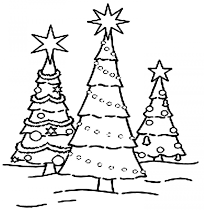
\includegraphics[width=0.25\textwidth]{img/drvca.png}
\end{wrapfigure}

Advent u Zagrebu tradicionalna je predblagdanska manifestacija koja se održava
na više lokacija u središtu Zagreba. Također valja istaknuti kako je upravo
ovaj događaj tri puta zaredom proglašen najboljom destinacijom za božićne
blagdane u Europi. Dobre vijesti brzo se šire pa je tako ova divna informacija
stigla i do sjevernog pola gdje živi Djed Božićnjak. Zanimljivo je da Djed
Božićnjak (osim poslovno na Badnju večer) nikada nije posjetio Hrvatsku. To je
donekle i logično jer je najveće uspjehe hrvatske nogometne reprezentacije
pratio u Francuskoj i Rusiji, ne voli sunce i more, a na COCI-ju se može bez
problema natjecati iz vlastitog doma.

Srećom, kucnuo je i taj čas, Djed Božićnjak je najavio čelnicima grada Zagreba
da će 14.\ prosinca sletjeti na Trg bana Jelačića. Najprije će prošetati do
Dalmatinske 12 gdje će (u neslužbenoj konkurenciji) sudjelovati na 3.\ kolu
HONI-ja, zatim će mu gospodin Malnar ukratko predstaviti gastronomsku ponudu
grada, potom će zajedno prošetati adventom, a kraj dana će dočekati kod
Žnidaršića.

Vjerojatno se pitate: ``Kako će točno djedica sletjeti na trg, pa tamo ne
postoji nikakva pista!''. U pravu ste, pista zasad ne postoji, ali to nije
velika prepreka. Naime, Milan je ionako htio na trg postaviti $N$ božićnih
drvca, a sada će ih samo rasporediti u dva retka te prostor između njih
proglasiti pistom. Gospodin Malnar se složio s tom idejom, ali također želi da
razlika u visini između svaka dva susjedna drvca u retku bude jednaka te da se
drvca uredno poslože od najnižeg ka najvišem. Pomozite Milanu i odredite neki
raspored drvca koji zadovoljava zahtjev gospodina Malnara.

%%%%%%%%%%%%%%%%%%%%%%%%%%%%%%%%%%%%%%%%%%%%%%%%%%%%%%%%%%%%%%%%%%%%%%
% Input
\subsection*{Ulazni podaci}
U prvom je retku prirodan broj $N$ $(2 \le N \le 10^5)$ iz teksta zadatka.

U sljedećem se retku nalazi $N$ prirodnih brojeva $h_i$ $(1 \le h_i \le 10^9)$
koji označavaju visine Milanovih božićnih drvca.

%%%%%%%%%%%%%%%%%%%%%%%%%%%%%%%%%%%%%%%%%%%%%%%%%%%%%%%%%%%%%%%%%%%%%%
% Output
\subsection*{Izlazni podaci}
U prvom retku ispišite prirodan broj $A$ koji predstavlja broj drvca koja će se
nalaziti u prvom retku piste. U drugom retku ispišite $A$ prirodnih brojeva koji
predstavljaju visine drvca prvog retka piste.

U trećem retku ispišite prirodan broj $B$ koji predstavlja broj drvca koja će se
nalaziti u drugom retku piste. U četvrtom retku ispišite $B$ prirodnih brojeva
koji predstavljaju visine drvca drugog retka piste.

Niti jedan redak drvca ne smije biti prazan $(A > 0$ i $B > 0)$ te svako drvce
mora biti u nekom retku $(A + B = N)$. Također, drvca u svakom retku trebaju
biti poredana od najnižeg ka najvišem. Ako postoji više mogućih rješenja,
ispišite bilo koje. Ako pak ne postoji ispravno rješenje, u jedini redak
ispišite -1.

%%%%%%%%%%%%%%%%%%%%%%%%%%%%%%%%%%%%%%%%%%%%%%%%%%%%%%%%%%%%%%%%%%%%%%
% Scoring
 \subsection*{Bodovanje}
{\renewcommand{\arraystretch}{1.4}
  \setlength{\tabcolsep}{6pt}
  \begin{tabular}{ccl}
 Podzadatak & Broj bodova & Ograničenja \\ \midrule
  1 & 20 & $N \le 15$ \\
  2 & 30 & $N \le 300$ \\
  3 & 30 & \makecell[l]{$M \le 10^5$,
            postoji rješenje u kojem su oba retka drvca jednako duga.
            } \\
  4 & 30 & Nema dodatnih ograničenja. \\
\end{tabular}}

%%%%%%%%%%%%%%%%%%%%%%%%%%%%%%%%%%%%%%%%%%%%%%%%%%%%%%%%%%%%%%%%%%%%%%
% Examples
\subsection*{Probni primjeri}
\begin{tabularx}{\textwidth}{X'X'X}
\sampleinputs{test/drvca.dummy.in.1}{test/drvca.dummy.out.1} &
\sampleinputs{test/drvca.dummy.in.2}{test/drvca.dummy.out.2} &
\sampleinputs{test/drvca.dummy.in.3}{test/drvca.dummy.out.3}
\end{tabularx}

%%%%%%%%%%%%%%%%%%%%%%%%%%%%%%%%%%%%%%%%%%%%%%%%%%%%%%%%%%%%%%%%%%%%%%
% We're done
\end{statement}

%%% Local Variables:
%%% mode: latex
%%% mode: flyspell
%%% ispell-local-dictionary: "croatian"
%%% TeX-master: "../hio.tex"
%%% End:
